\documentclass[a4paper,10pt]{article}
\usepackage[utf8x]{inputenc}
\usepackage[slovene]{babel}
\usepackage{amsmath}
\usepackage{amsfonts}
\usepackage{relsize}
\usepackage[smaller]{acronym}
\usepackage{graphicx}
\usepackage{subfigure}
\usepackage{cite}
\usepackage{url}
\usepackage{hyperref}

\renewcommand{\theta}{\vartheta}
\renewcommand{\phi}{\varphi}

\newcommand{\dd}{\,\mathrm{d}}

\title{Fourierova analiza}
\author{Miha \v Can\v cula}

\begin{document}
  \maketitle

\begin{figure}[h]
  \centering
  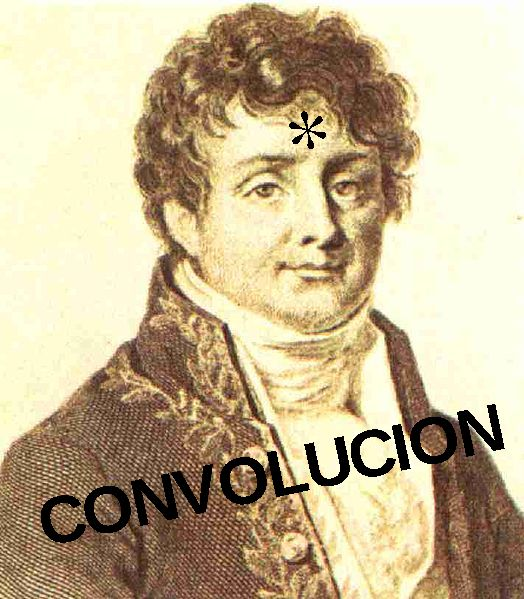
\includegraphics[width=.5\textwidth]{Convolucion}
  \caption{Znani francoski konvolucionar Jean Baptiste Joseph Fourier}
\end{figure}

\section{Konvolucija}

Linearno padajo"co funkcijo $f(x) = 1-x$ sem izvrednostil v $N$ diskretnih to"ckah, nato pa numeri"cno ra"cunal konvolucijo te funkcije samo s sabo. Ta ra"cun sem ponovil pri razli"cnih vrednostih $N$ in ga vsakih napravil na dva na"cina: enkrat po definiciji konvolucije, drugi"c pa z uporabo Fourierove transformacije. Za vse ra"cune sem uporabil program \texttt{GNU Octave}. 

\subsection{Hitrost}

Z grafa na sliki~\ref{fig:konv-cas}, se vidi, da je Fourierova transformacija mnogo hitrej"sa od direktnega ra"cuna konvolucije, ta razlika pa se vidi predvsem pri velikem "stevilu to"ck $N$. 

\begin{figure}[h]
 \centering
\input{g_konv_cas}
\caption{"Cas, potreben za izra"cun konvolucije treh linearno padajo"cih funkcij po obeh algoritmih}
\label{fig:konv-cas}
\end{figure}

Na grafu sta narisani "se ujemanju s krivuljo, ki nara"s"ca kot $\cal O(n^2)$ in krivuljo $\cal O(n\log n)$. V obeh primerih sem funkcijama dodal konstanto, saj "ze sam program \texttt{Octave} potrebuje nekaj "casa za zagon. Ujemanje je dobro za obe napovedi, predvsem pri ve"cjih $N$, ko lahko zanemarimo prispevke ni"zjih redov. 

\subsection{Natan"cnost}

Preveril sem tudi, kako natan"cna je metoda s Fourierovo transformacijo. Tako direktna kot FFT metoda ne delata nobenih pribli"zkov, edini vir napake je kon"cna natan"cnost ra"cunalni"skega zapisa, na katerege pa sta lahko metodi razli"cno ob"cutljivi. Kot mero za napako metode sem izbral

\begin{align}
 \sigma^2 &= \sum_{i=0}^{kN-1} (f_i^F - f_i^D)^2
\end{align}

kjer so $f_i^F$ in $f_i^D$ koeficienti, izra"cunani s Fourierovo oz. direktno metodo. "Ce sem za"cel z diskretizacijo na $N$ to"ck in izra"cunal konvolucijo $k$-tih enakih funkcij, ima kon"cni izraz $kN$ koeficientov. 


\begin{figure}[h]
 \centering
\input{g_konv_napaka}
\caption{Napaka izra"cuna s Fourierovo transformacijo}
\end{figure}

\section{Dekonvolucija signala}

Tokrat je bila naloga obratna, poiskati izviren signal ob poznavanju izhodnega signala in prehodne funkcije. Prehodna funkcija $G(t)$ pa je imela en neznani parameter $\beta$, ki sem ga dolocil tako, da je bil izvirni signal "cim lep"si. Lepoto signala pa sem definiral na razli"cne na"cine. 

\begin{figure}[h]
 \input{g_decon_3d}
 \caption{Izra"cunani izvirni signal z upo"stevanjem razli"cnih eksponentov $\beta$}
\label{fig:decon-3d}
\end{figure}


\subsection{"Cim manj"se spremembe}

Ena mo"zna izbira je, da i"s"cemo signal, ki se "cim po"casneje spreminja. Naravna izbira je tak"sna, da je izraz

\begin{align}
  \sum_{i=0}^{N-1} \left| s_i - s_{i-1}\right|^2
\end{align}

"cim manj"si. Izka"ze se, da je to pri vrednosti $\beta = 34.852$, vhodni signal pa je tedaj tak kot na sliki~\ref{fig:dekon-signal}. 

\begin{figure}[h]
 \input{g_decon_signal}
\caption{Vhodni in izhodni signal pri $\beta = 34.852$}
\label{fig:dekon-signal}
\end{figure}

\subsection{"Cim ni"zje frekvence}

Lepoto signala pa lahko ocenimo "ze po frekven"cnem spektru, tako da si "zelimo "cim manj visokih frekvenc. V ta namen sem minimiziral izraz

\begin{align}
 \sum_{i=-N/2}^{N/2-1} i\cdot|S_i|
\end{align}

kjer so $S_i$ komponentne Fourierove transformacije signala $s_i$. Ta kriterij je v bistvu zelo podoben prej"snjemu, zato je tudi optimalna vrednost $\beta$ blizu, in sicer $\beta = 36.475$. 

\subsection{"Cim manj"sa amplituda}

Za primerjavo sem iskal tudi signal z najmanj"so amplitudo. "Ce privzamemo, da je signal pribli"zno sinusen, lahko njegovo amplutido ocenimo v vsaki to"cki. 

\begin{align}
 s(t) &= A\sin \omega t \\
 \dot s(t) &= A\omega \cos \omega \\ 
 A^2 &= \omega^2 s^2 + (\dot{s})^2
\end{align}

Odvod $\dot s$ lahko pribli"zamo s kon"cno diferenco, frekven"co $\omega$ pa kot po absolutni vrednosti najve"cjo komponentno Fourierove transformiranke. Seveda na"s signal ni povsem sinusen, zato se amplituda spreminja s "casom, $A = A(t)$. Podobno kot v prvem primeru sem na koncu minimiziral povpre"cen kvadrat amplitude. 

\section{Filtriranje}

\subsection{Celoten interval}

Iz frekven"cnega spektra originalnih signalov na sliki~\ref{fig:val-fft} lahko vidimo, da sta oba vrhova v spektru signala iz datoteke \texttt{val2.dat} ostra, medtem ko so vrhovi v spektru \texttt{val3.dat} raz"sirjeni. Iz tega lahko sklepamo, da smo pri merjenju prvega signala ujeli celo "stevilo period, pri merjenju drugega pa ne. 

\begin{figure}[h]
 \input{g_val_fft}
\caption{Frekven"cni spekter obeh signalov}
\label{fig:val-fft}
\end{figure}

Oba spektra lahko pribli"zamo z uporabo okenske funkcije. Najprej sem poskusil z enostavno sinusno funkcijo

\begin{align}
 w(n) &= \sin(\frac{n\pi}{N-1})
\end{align}

Ta funkcija se na robovih dotakne 0, ima pa neni"celen odvod. Frekven"cni spekter obeh signalov, pomno"zenih s tak"snim oknom, je na sliki~\ref{fig:val-cos}. 

\begin{figure}[h]
 \input{g_val_cos}
\caption{Frekven"cni spekter obeh signalov, pomno"zenih s sinusno okensko funkcijo}
\label{fig:val-cos}
\end{figure}

Hitro vidimo, da so se vrhovi prej ostrega signala ra"zsirili, vrhovi signala s "sirokimi vrhovi pa zo"zili. Med signaloma je "se vedno jasna razlika, vrhovi so po "sirini sedaj bolj podobni kot prej, ne pa "se enaki. 

Nato sem preizkusil Hammingovo okensko funkcijo. Za razliko od prej"snje ta niti na robovih ne pade "cisto na 0, ima pa tam odvod enak 0, zato bo tako obdelan signal lahko zvezen in periodi"cen. Koeficiente okna dobimo s formulo

\begin{align}
 w(n) &= 0.54 - 0.46 \cos \left(\frac{2\pi n}{N-1}\right)
\end{align}

"Ce okensko funkcijo uporabimo v Fourierovem prostoru, je predznak drugega "clena odvisen od izbire intervala za $n$. V tem primeru pa smo jo uporabili v "casovnem prostoru, tako da $n \in [0,N-1]$ in je drugi "clen s pozitivnim predznakom. "Zelimo namre"c, da je vrednost okna na robovih intervala enaka 0, na sredini pa 1.  Rezultat uporabe zgornje funkcije je na sliki~\ref{fig:val-hamm}. 

\begin{figure}[h]
 \input{g_val_hamm}
\caption{Frekven"cni spekter obeh signalov, pomno"zenih s Hammingovo okensko funkcijo}
\label{fig:val-hamm}
\end{figure}

"Sirini vrhov pa sta skoraj enaki. Na sliki je sicer vidna razlike med njimi, ampak le v podro"cju med vrhovi, kjer je spekter sedaj mnogo ni"zji kot pri izvirnem signalu. Opazimo lahko tudi, da v signalu \texttt{val3.dat} tik ob najvi"sjih vrhovih sedaj dobimo skoke (angl. side-lobes), "ceprav je Hammingova funkcija optimizirana tako, da "cimbolj zmanj"sa vi"sino prvega skoka. 

Nazadnje sem uporabil se Blackmanovo funkcijo, ki ima na robovih tako vrednost kot odvod enaka 0. Rezultati so na sliki~\ref{fig:val-black}. 

\begin{figure}[h]
 \input{g_val_black}
\caption{Frekven"cni spekter obeh signalov, pomno"zenih z Blackmanovo okensko funkcijo}
\label{fig:val-black}
\end{figure}

\cleardoublepage
\subsection{Kraj"si intervali}

Ogledal sem si tudi, kaj se zgodi, "ce obravnavamo le manj"se "stevilo to"ck. Iste izra"cune kot prej sem ponovil za celoten signal (512 to"ck) in za kraj"se podintervale (64, 128 in 256 to"ck). Tokrat sem prikazal le originalen signal in pa signal, dobljen s Hammingovo okensko funkcijo. Spektri so na slikah~\ref{fig:val-dolzina} in~\ref{fig:val-dolzina-hamm}. 

\begin{figure}[h]
 \subfigure[$M = 64$]{\input{g_val_64}\label{fig:val-dolzina-64}} 
 \subfigure[$M = 128$]{\input{g_val_128}}
 \subfigure[$M = 256$]{\input{g_val_256}}
 \subfigure[$M = 512$]{\input{g_val_512}}
\caption{Frekve"cni spektri originalnih signalov pri razli"cnih dol"zinah analiziranega intervala}
\label{fig:val-dolzina}
\end{figure}

Okenska funkcija "ze pri manj"sem "stevilu to"ck poskrbi, da so vrhovi bolje razlo"cni tudi na logaritemski sliki, poleg tega pa so tudi po obliki bolj podobni med seboj. Njen vpliv dobro viden pri $M=64$, na sliki~\ref{fig:val-dolzina-64} sta vrhova modre funkcije vidno razli"cno "siroka, medtem ko sta njuni "sirin na sliki~\ref{fig:val-dolzina-hamm-64}a pribli"zno enaki. 

\begin{figure}[h]
 \subfigure[$M = 64$]{\input{g_val_hamm_64}\label{fig:val-dolzina-hamm-64}} 
 \subfigure[$M = 128$]{\input{g_val_hamm_128}}
 \subfigure[$M = 256$]{\input{g_val_hamm_256}}
 \subfigure[$M = 512$]{\input{g_val_hamm_512}}
\caption{Frekve"cni spektri signalov, pomno"zenih s Hammingovo okensko funkcijo, pri razli"cnih dol"zinah analiziranega intervala}
\label{fig:val-dolzina-hamm}
\end{figure}



\end{document}
